%!TEX root = ttc15-train-benchmark-sigma.tex

\section{Constraints}
\label{sec:Constraints}

In the following we describe the individual constraints that were part of the case study (case study tasks) except the \emph{PosLength} and \emph{SwitchSet} which have already been shown above (\Cf Section~\ref{sec:SolutionDescription}).

\begin{itemize}[---]
  \item \emph{SwitchSensor}
  %
  \begin{scalacode}
  BooleanConstraint[Switch](
    query = switch => switch.sensor.isEmpty,
    repair = switch => switch.sensor = Sensor()
  )
  \end{scalacode}
  %
  The \texttt{isEmpty} is a method that is defined on an \texttt{Option} type (coming from the standard Scala library) representing a type which may or may not have a value.
  Since in the model, the \emph{sensor} reference of the \texttt{Switch} class is defined as optional (with cardinality \texttt{0..1}), in \SIGMA we represent the reference using the \texttt{Option} class.
  Not only makes this the cardinality expressed in the type definition, but it also prevents some of the \texttt{NullPointerException}s caused by traversing unset references.
  Technically, this is realized by implicit conversions (\Cf Krikava~\Etal \cite{Krikava2014}).

  \item \emph{RouteSensor}
  %
  \begin{scalacode}
  Constraint[Route, (Route, Sensor, SwitchPosition, Switch)](
    query = route => {
      for {
        swP <- route.follows
        sw = swP.switch
        sensor <- sw.sensor if !(route.definedBy contains sensor)
      } yield (route, sensor, swP, sw)
    },

    repair = {
      case (route, sensor, _, _) => route.definedBy += sensor
    }
  )
  \end{scalacode}
  %
  The implementation is similar to the the previous case.
  It is also based on a for comprehension and closely follows the description of the query.
  
  \item \emph{SemaphoreNeighbor}
  %
  \begin{scalacode}
  Constraint[Route, (Semaphore, Route, Route, Sensor, Sensor, TrackElement, TrackElement)](
    query = route1 => {
      for {
        sensor1 <- route1.definedBy if route1.exit != null
        te1 <- sensor1.elements
        te2 <- te1.connectsTo
        sensor2 <- te2.sensor
        route2 <- sensor2.sContainer[Route] if route1 != route2
        semaphore = route1.exit if semaphore != route2.entry
      } yield (semaphore, route1, route2, sensor1, sensor2, te1, te2)
    },

    repair = {
      case (semaphore, _, route2, _, _, _, _) => route2.entry = semaphore
    }
  )
  \end{scalacode}
  %
  Again based on the for comprehension.
  Additionally, we provide a shortcut using the \texttt{route1.exit != null} so immediately skip the route instances that do not have an exit semaphore set. 

\end{itemize}

The complete solution is implemented in a Scala object\footnote{A Scala object defines a single instance of a class.} \texttt{hu.bme.mit.trainbenchmark.ttc. benchmark.sigma.Solution}.

\section{Integration with the Train Benchmark Framework}
\label{sec:SchemaIntegration}

Figure~\ref{fig:IntegartionSchema} shows the various layers of integration of the solution into the train benchmark framework.

\begin{figure}[h!tb]
  \centering
  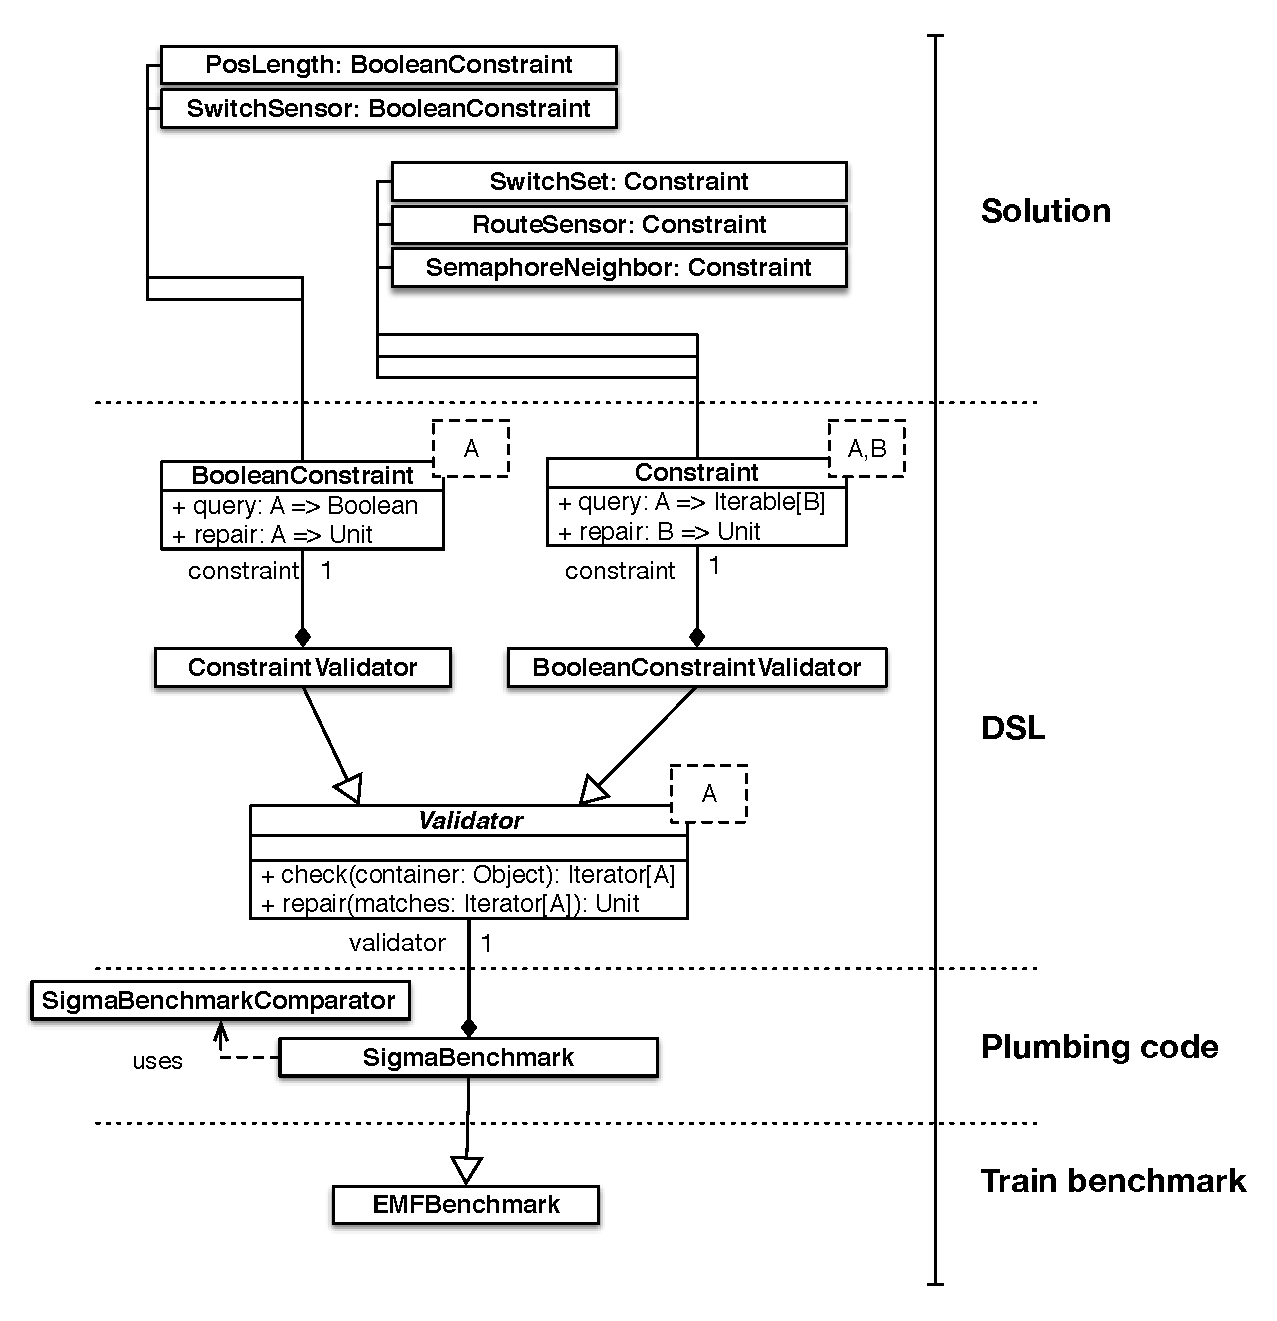
\includegraphics[width=\textwidth]{figures/integration.pdf}
  \caption{Integration schema}
  \label{fig:IntegartionSchema}
\end{figure}


\section{Performance Comparison}
\label{sec:PerformanceComparison}

The following charts have been generated by the case study benchmark.
They present a performance comparison between \SIGMA and the reference implementation in Java on the model instances from size 1 to 8192 using 8GB memory dedicated to the JVM.
The corresponding results are shown in the figures~\ref{fig:SigmaFixedValidationBatch} and~\ref{fig:SigmaFixedReValidationBatch}.
We compare them to the Java solution which is shown in the figures~\ref{fig:JavaFixedValidationBatch} and~\ref{fig:JavaFixedReValidationBatch}.

\begin{figure}[h!tb]
  \centering
  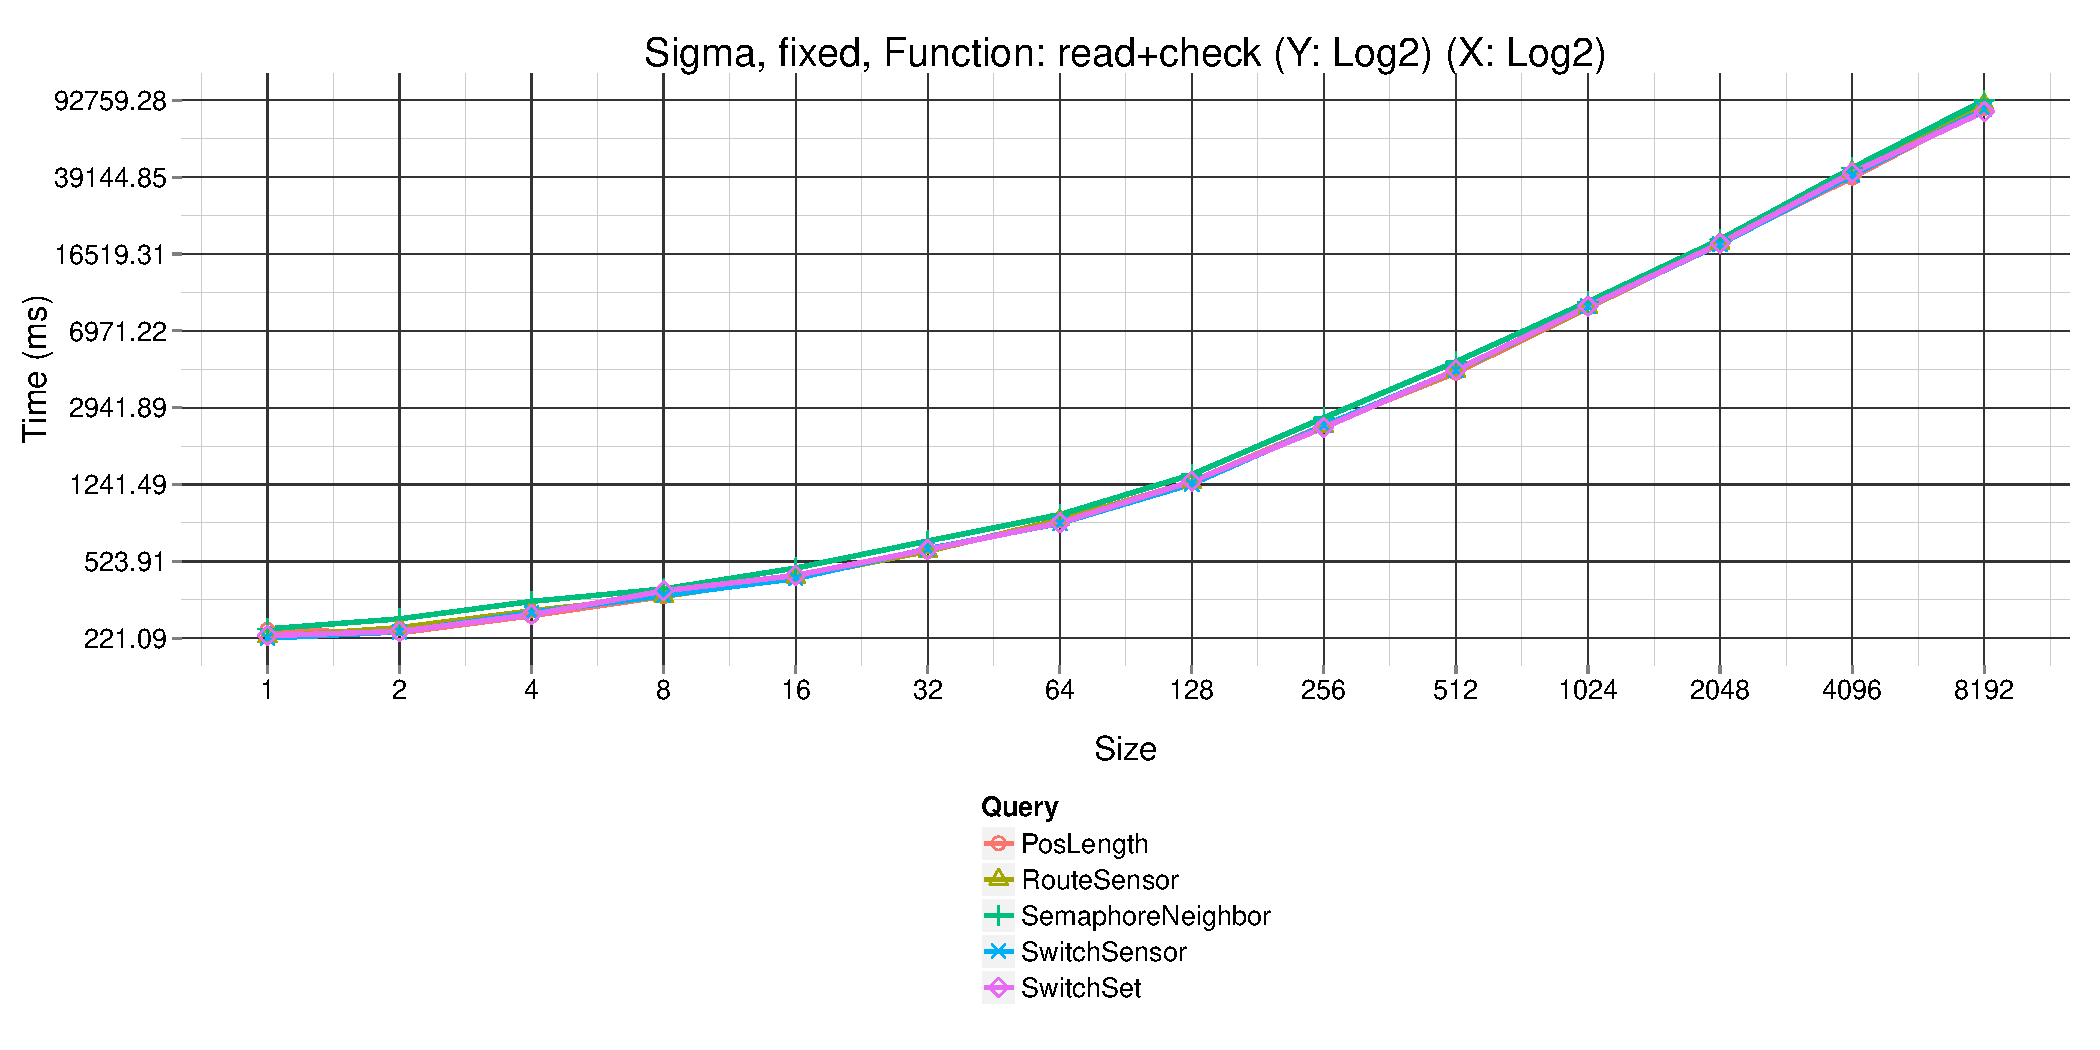
\includegraphics[width=\textwidth]{figures/fixed-Sigma-GroupBy-Query-time-batch-validation.pdf}
  \caption{\SIGMA fixed validation batch}
  \label{fig:SigmaFixedValidationBatch}
\end{figure}

\begin{figure}[h!tb]
  \centering
  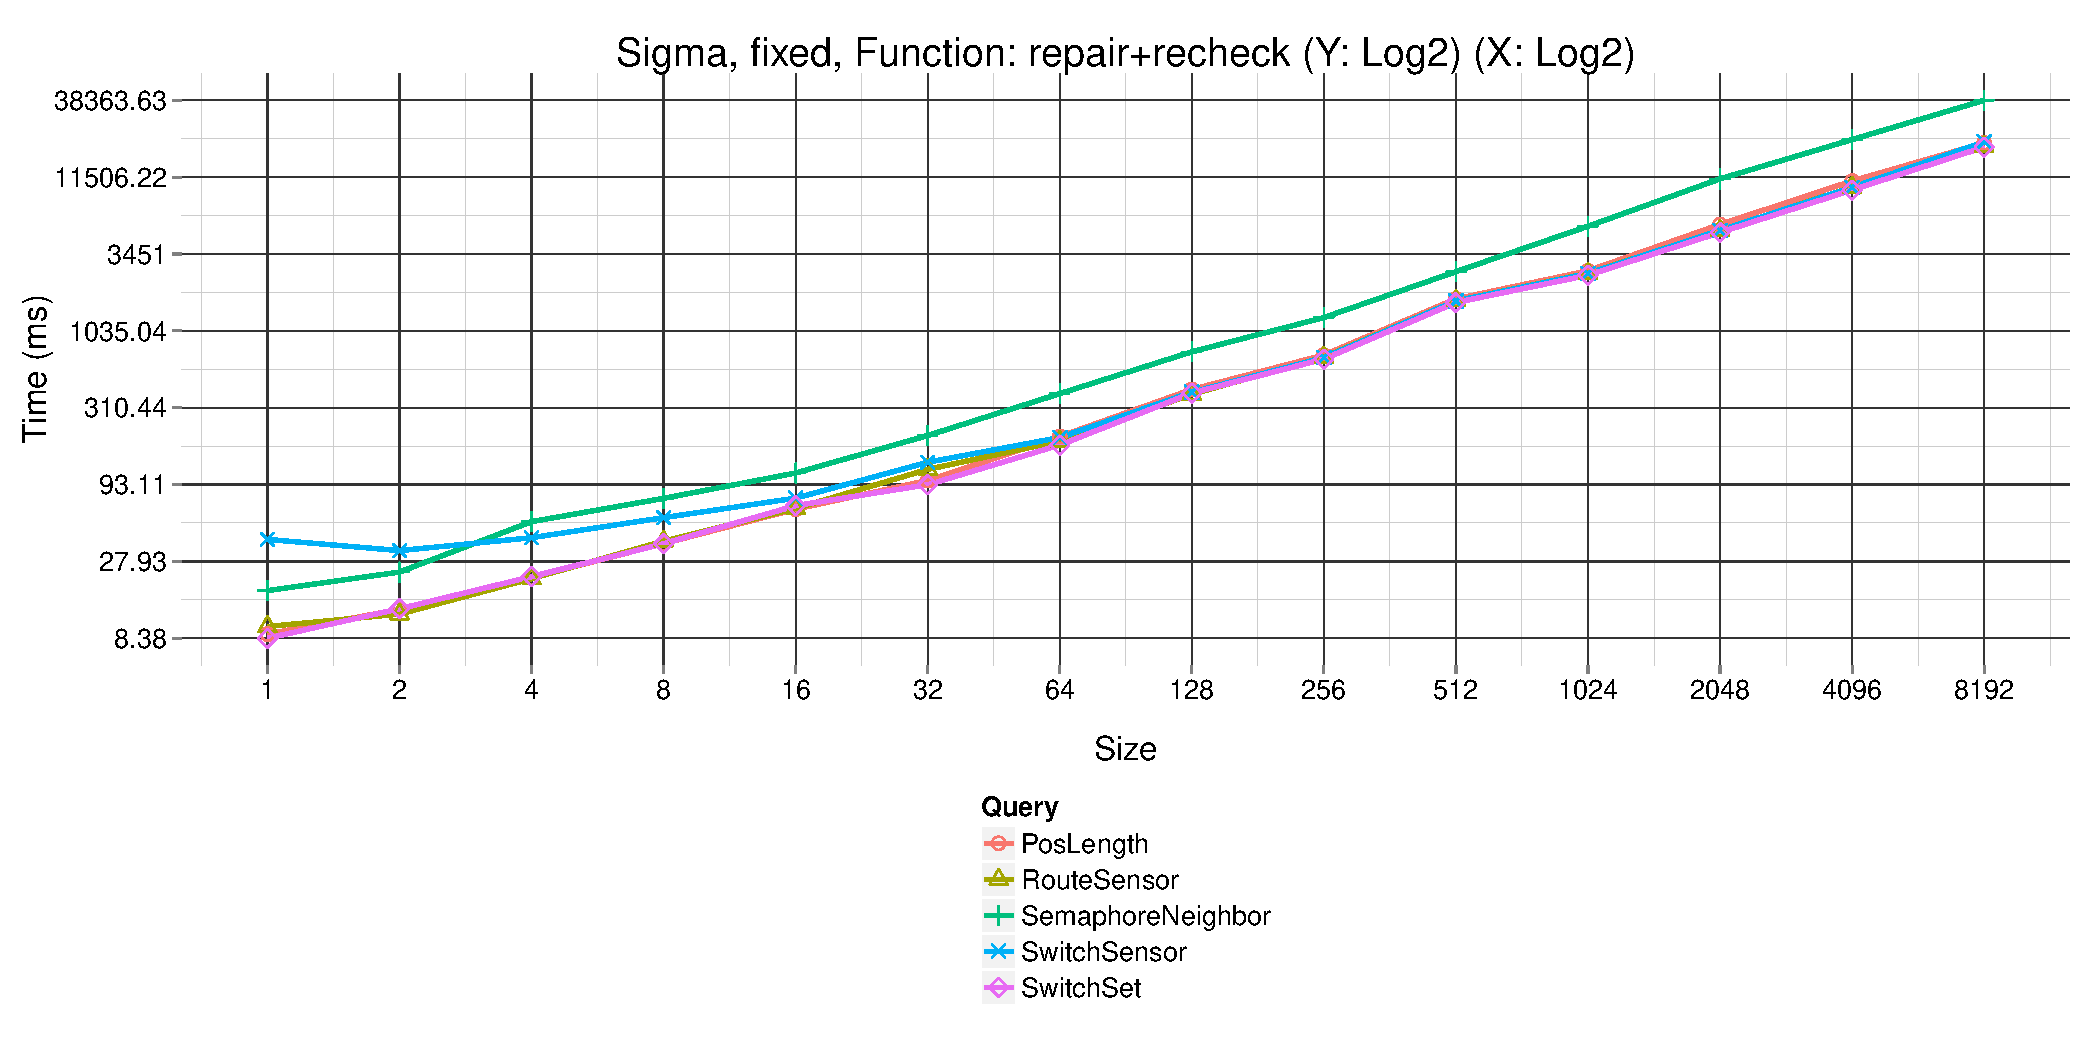
\includegraphics[width=\textwidth]{figures/fixed-Sigma-GroupBy-Query-time-revalidation.pdf}
  \caption{\SIGMA fixed revalidation}
  \label{fig:SigmaFixedReValidationBatch}
\end{figure}

\begin{figure}[h!tb]
  \centering
  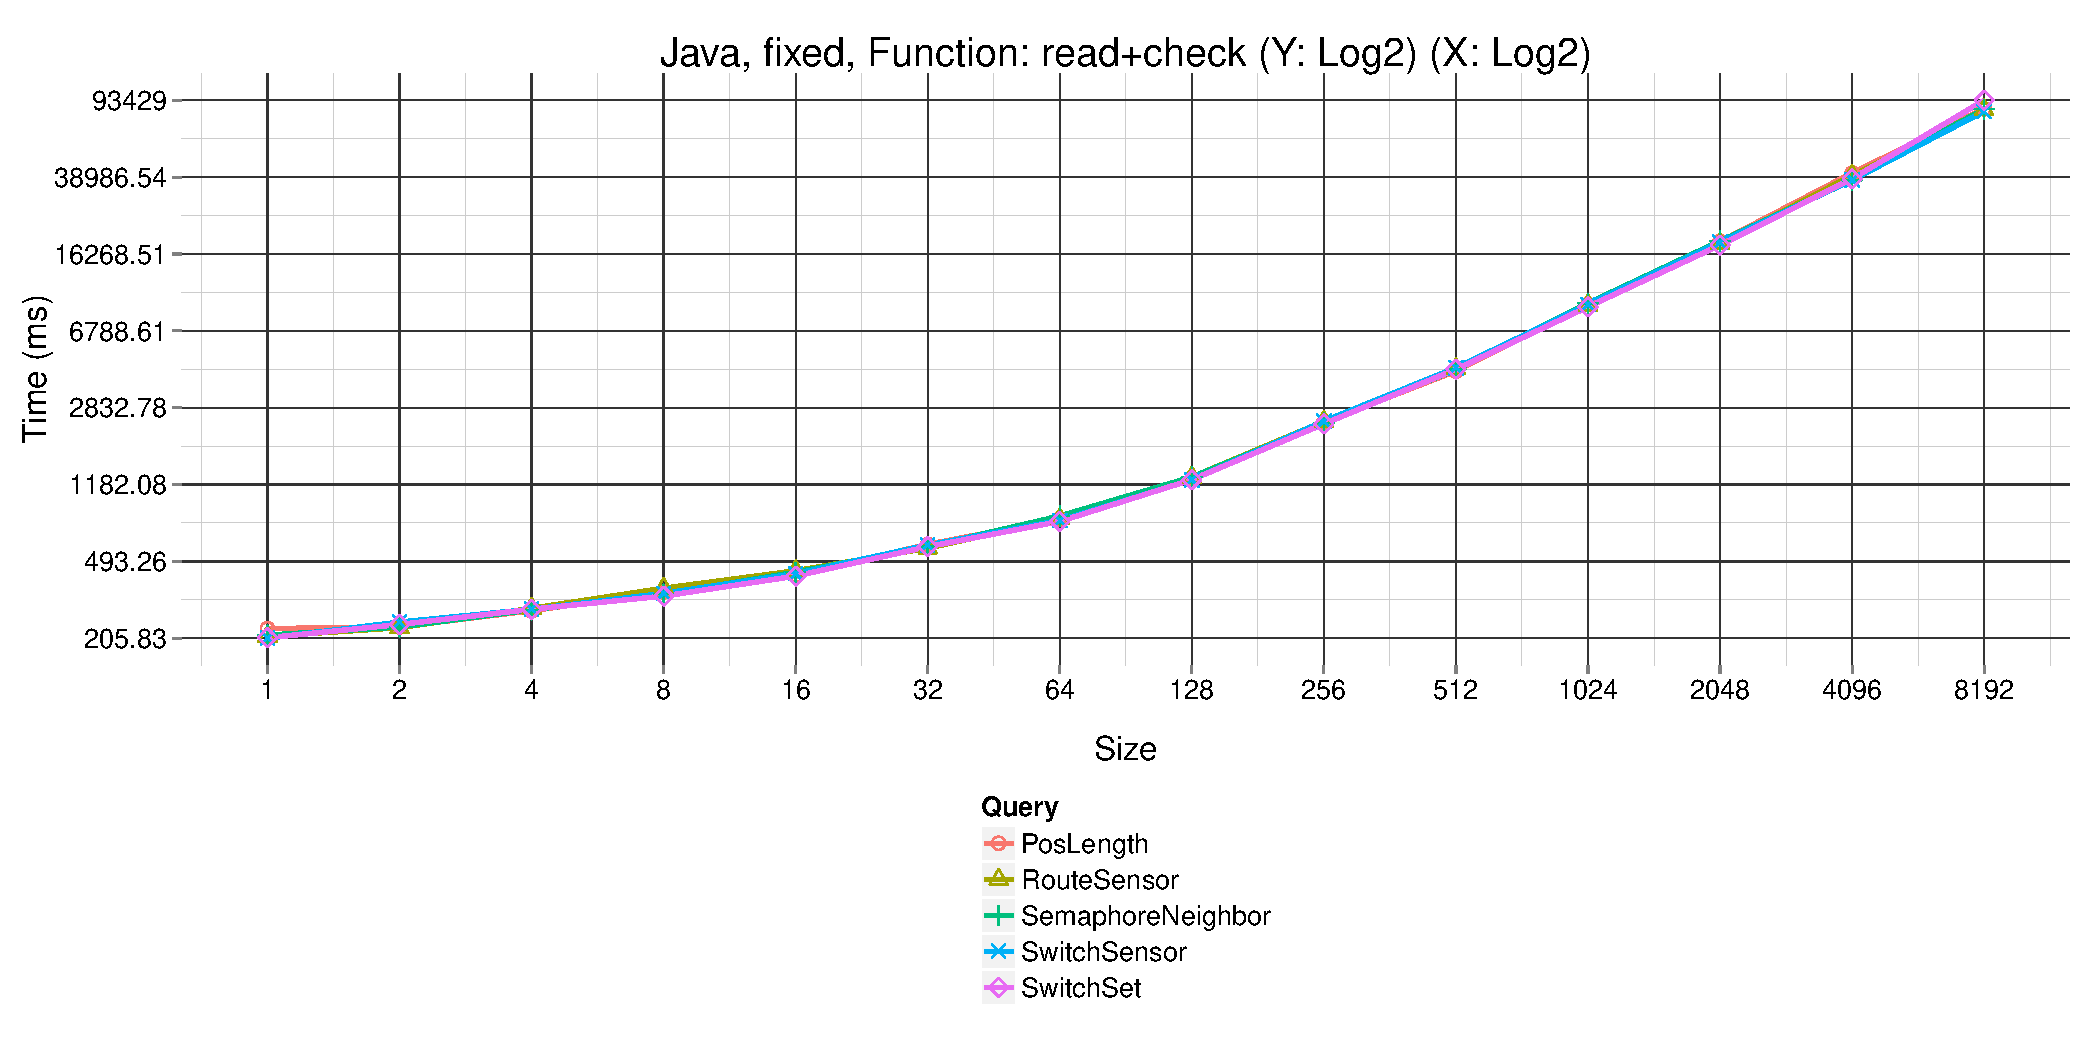
\includegraphics[width=\textwidth]{figures/fixed-Java-GroupBy-Query-time-batch-validation.pdf}
  \caption{Java fixed validation batch}
  \label{fig:JavaFixedValidationBatch}
\end{figure}

\begin{figure}[h!tb]
  \centering
  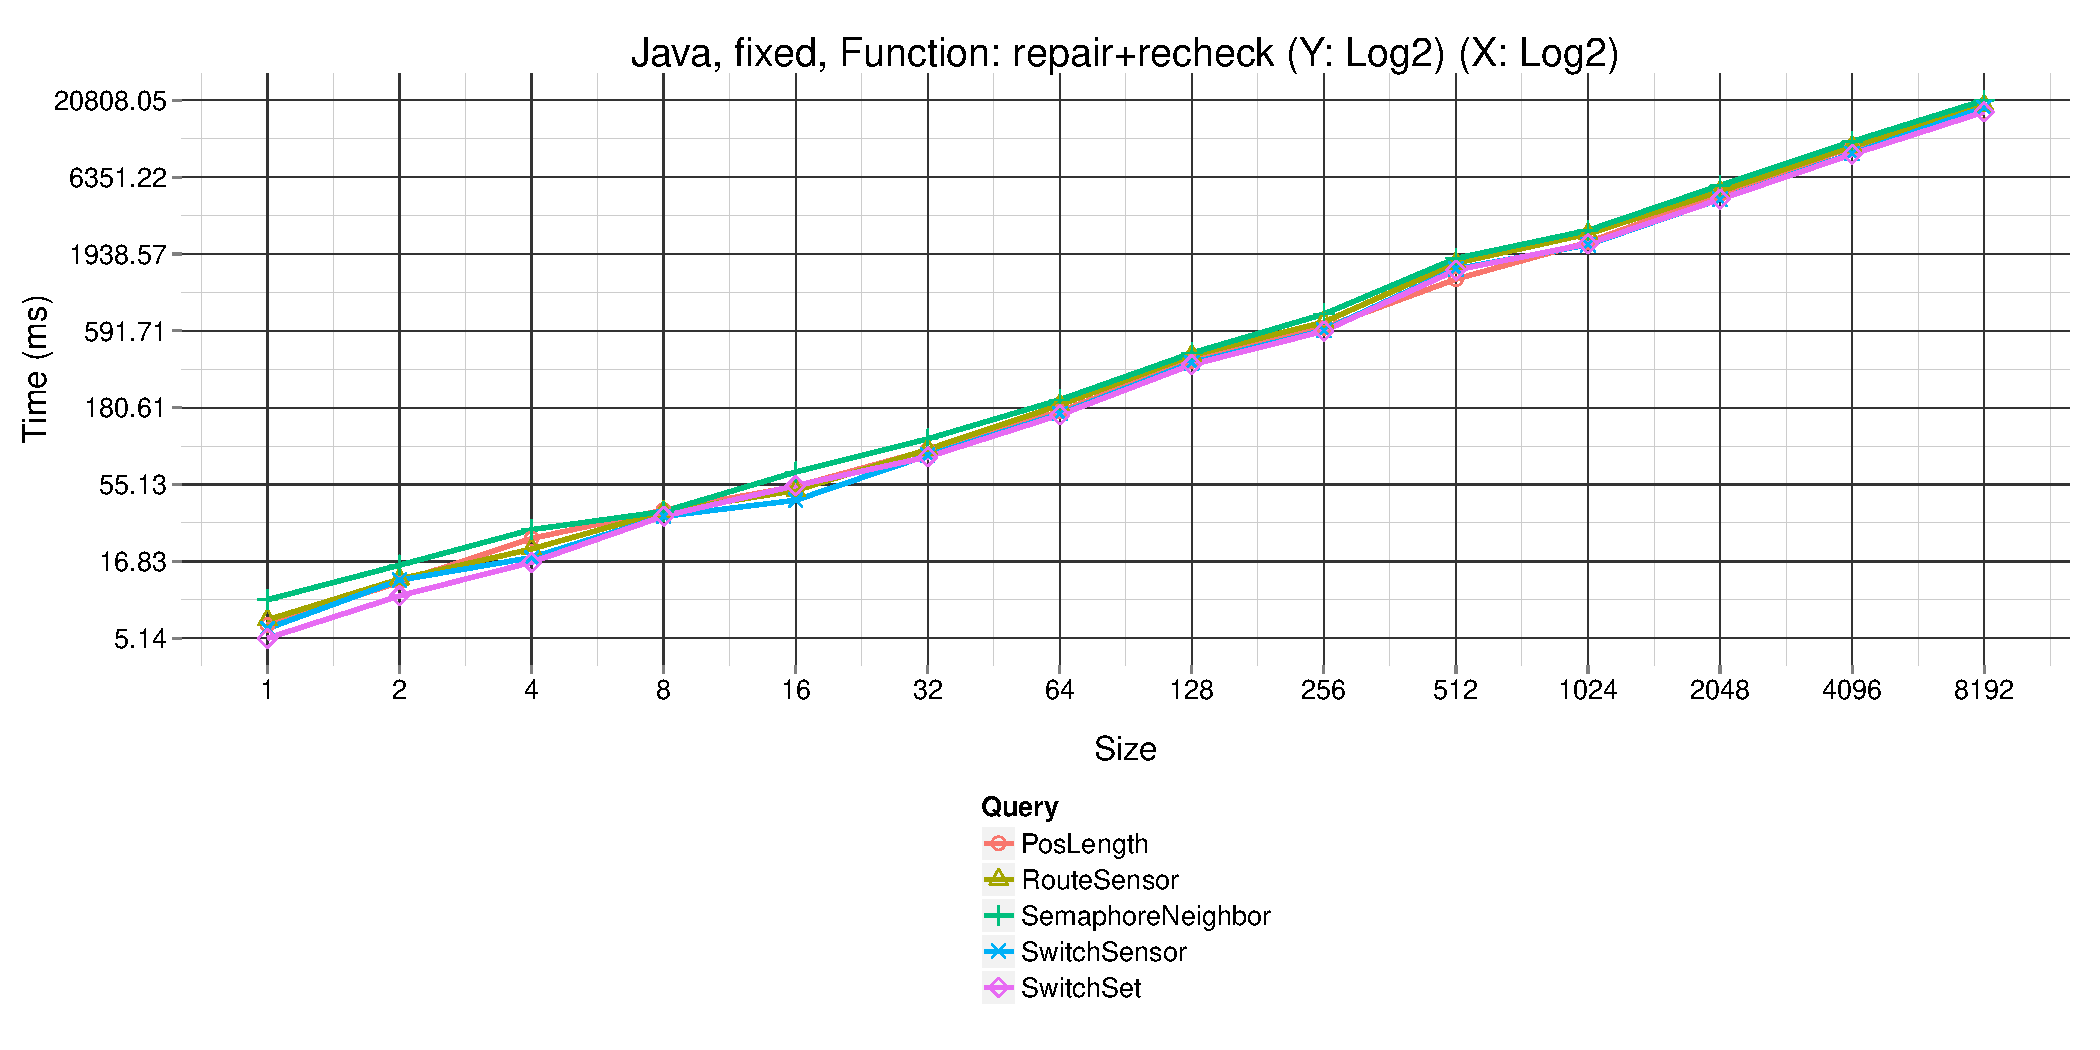
\includegraphics[width=\textwidth]{figures/fixed-Java-GroupBy-Query-time-revalidation.pdf}
  \caption{Java fixed revalidation}
  \label{fig:JavaFixedReValidationBatch}
\end{figure}